\chapter{Численная схема решения}
Поставленная задача (\ref{eq1:system}), так как является достаточно сложной системой нелинейных дифференциальных уравнений, решается с помощью численного моделирования. 
Сформулированное  уравнение  (\ref{eq1:system})  с  соответствующими краевыми  условиями  (начальными и  граничными)  решается численно, методом конечных разностей (МКР).

\section{Сеточная функция} \label{grid}
Для аппроксимации системы дифференциальных уравнений (\ref{eq1:system}) разностным методом для начала введем пространственно - временную сетку на плоскости $x = (x_{1},x_{2})$ с координатами $x^{i}_{1} = i \cdot h_{1},\; x^{j}_{2} = j \cdot h_{2} , \; t^{k} = k \cdot \tau $, где $h_{1},\; h_{2}$ -- шаги по пространству, $\tau$ - шаг по времени; $i = \overline{0,N}, j = \overline{0,M}$ и $k = \overline{0,T}$. Таким образом, вся расчетная область покрывается сеткой (рис. \ref{fig:grid}).

\begin{figure}[ht]
    \centering
    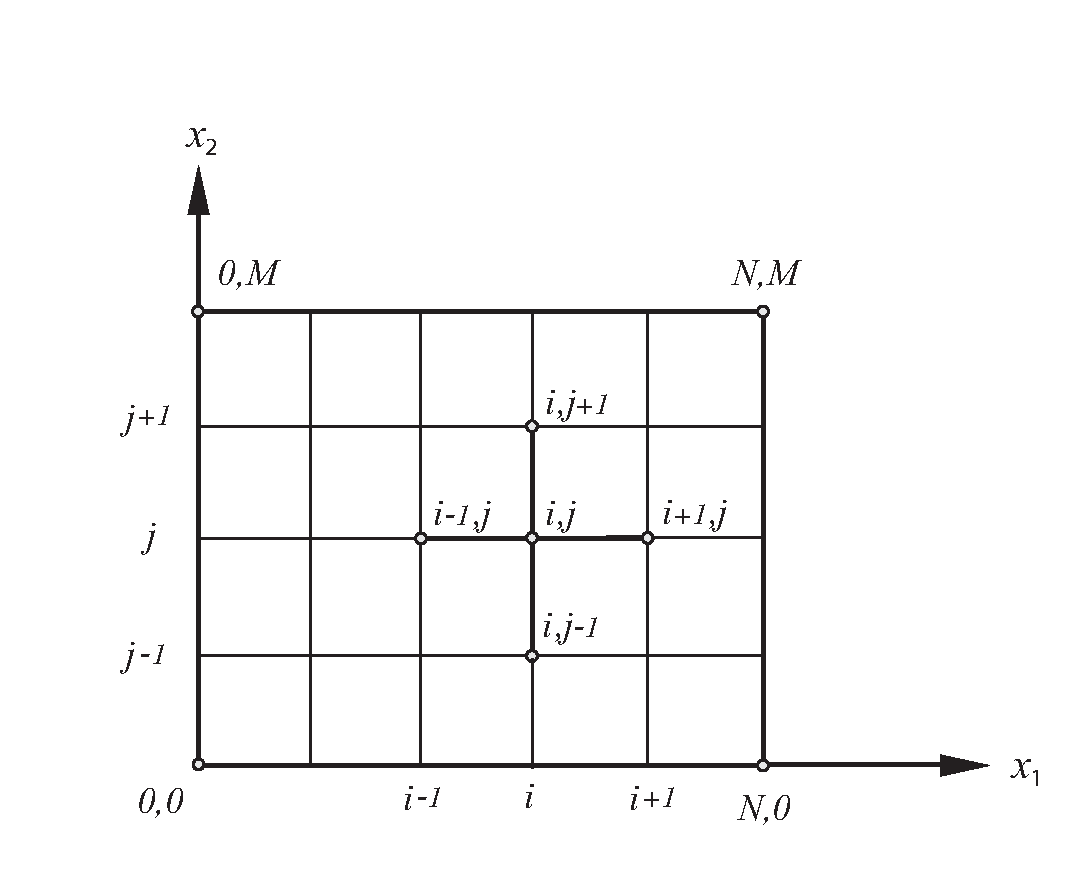
\includegraphics[scale = 0.5]{grid}
    \captionsetup{justification=centering,margin=2cm}
    \caption{Разностная сетка области решения}
    \label{fig:grid}
\end{figure}

 Узлы которые попали внутрь $\Omega$, назовем \textit{внутренними}, а их совокупность обозначим $\omega_{h}$. Точки пересечения прямых $x^{i}_{1} = i \cdot h_{1}$ и $x^{j}_{2} = j \cdot h_{2}$ с границей $\Gamma$ назовем \textit{граничными}, а множество всех граничных узлов обозначим $\gamma_{h}$.
 
 И так, область изменения аргумента $x = (x_{1},x_{2})$ заменяется сеткой  $ \overline{\omega_{h}} = \omega_{h} + \gamma_{h}$, то есть конечным множеством точек $x^{i}_{1}, x^{j}_{2}$, принадлежащих $\overline{\Omega} = \Omega + \Gamma$. И вместо функции $u(x_{1},x_{2},t)$ непрерывного аргумента $x \in \overline{\Omega} $ будем рассматривать сеточные функции $y(x^{i}_{1},x^{j}_{2},t^{k})$ \cite[Самарский][67]{Samarskiy1977}.

\section{Разностная аппроксимация уравнения}

Система (\ref{eq1:system}) состоит из дифференциальных уравнений одного типа, поэтому для удобства описания численной схемы решения, воспользуемся лишь одним уравнением, с соответствующими краевыми условиями: 

\begin{empheq}[left=\empheqlbrace]{align}
    \label{eq2:diffusion}
    &\frac{\p u} {\p t} = Lu + F, \qquad x \in \Omega, \qquad x = (x_{1},x_{2}) \\
    \label{eq2:cond}
    &\left.\left(A u + K \frac{\partial u}{\partial n} \right) \right|_{\Gamma } =\varphi, \qquad x \in \; \Gamma, \quad A = const.\\
    \label{eq2:init}
    &u(x,t)\vert_{t=0} =u_{0}(x)
\end{empheq}

При написании разностной схемы первым шагом является аппроксимация дифференциального оператора $L = \nabla \left(K \cdot \nabla \right)$. Пусть 
\begin{equation}
        \Lambda y = \Lambda_{1} y + \Lambda_{2} y,
        \qquad \Lambda_{\alpha} y = \frac{\p }{\p x_{\alpha}} \left(\mu \frac{\p y}{\p x_{\alpha}} \right),
        \qquad \alpha = 1,2,
\end{equation}
--- пятиточечный оператор на $\omega_{h}$ с шагами $h_{1}$ и $h_{2}$.
Таким образом дифференциальный оператор $L_{\alpha}$ заменяем разностным $\Lambda_{\alpha}$.

Для численного решения задачи (\ref{eq2:diffusion} ), воспользуемся \textit{неявной} схемой переменных направлений. Эту схему часто называют \textit{схемой Писмена - Рекфорда}\cite{peaceman}. 

\subsection{Метод переменных направлений}
 Дискретизация уравнения (\ref{eq2:diffusion}) проводится на основе локально-одномерной схемы для уравнений с переменными коэффициентами \cite[Самарский,][529]{Samarskiy1977}, которая является абсолютно устойчивой (при любых $\tau$ и $h$) и обладает свойством суммарной аппроксимации имея порядок точности $O(\tau + h^{2})$. Основная идея этого метода состоит в сведении перехода со слоя на слой к последовательному решению одномерной задачи вдоль строк и вдоль столбцов.
 
Введем следующее обозначение: $y(x^{i}_{1},x^{j}_{2},t^{k}) = y^{k}_{i,j}$. И так шаг по времени реализуется в два этапа --- на промежуточном временном шаге (полушаге)  $t = t^{k+1/2}$ проводим дискретизацию двумерного уравнения (\ref{eq2:diffusion}) только в направлении оси $Ox_{1}$ и получаем одномерное уравнение, после его решения вновь проводим дискретизацию уравнения (\ref{eq2:diffusion}), но уже в направлении оси $Ox_{2}$ и, решая полученное одномерное уравнение, определяем значение на целом временном шаге $t = t^{k+1}$.
\begin{empheq}{align}
		\frac{y^{k+1/2}_{i,j} - y^{k}_{i,j}}{0.5\tau} &= \Lambda_{1} y^{k+1/2}_{i,j} + f^{k}_{i,j} \label{eq2:los1},\\[2.5pt]
		\frac{y^{k+1}_{i,j} - y^{k+1/2}_{i,j}}{0.5\tau} &= \Lambda_{2} y^{k+1}_{i,j} + f^{k}_{i,j} \label{eq2:los2}.
\end{empheq}

Коэффициенты диффузии $K = K(u,v)$ зависят от неизвестных функции, поэтому для аппроксимации локально одномерных задач (\ref{eq2:los1}) - (\ref{eq2:los2}) воспользуемся методом баланса (интегро-интерполяционный метод) \cite[571]{Tihonov}. 

\subsection{Метод баланса} \label{ssec:balance}

В виду того что решается одномерное уравнение, опустим индексирование по одному из аргументов, а промежуточное значение функции при $t=t^{k+1/2}$, для упрощения записи, обозначим как  $y^{k+1/2}_{i,j} = \overline{y}_{i,j}$.

На отрезке $x_{i-1/2} \leq x \leq x_{i+1/2}$ где $x_{i-1/2} = \frac{1}{2}(x_{i-1} + x_{i})$ за время $\Delta t/2$ проинтегрируем локально одномерные уравнения, полученные из исходного уравнения (\ref{eq2:diffusion}):

\begin{gather}
    \int\limits_{x_{i-1/2}}^{x_{i+1/2}} \left(\overline{y}_{i} - y^{k}_{i}\right)dx = 
    \int\limits_{t^k}^{t^{k+\tau/2}} \Big(W_{i+1/2} - W_{i-1/2}\Big)dt +
    \int\limits_{t^k}^{t^{k+\tau/2}} \int\limits_{x^{i-1/2}}^{x^{i+1/2}} f_{i}\,dx\,dt \\[2pt]
    W_{i+1/2} = \mu_{i+1/2} \bigg( \frac{\overline{y}_{i+1} - \overline{y}_{i}}{h} \bigg) , \quad
	W_{i-1/2} = \mu_{i-1/2} \bigg( \frac{\overline{y}_{i} - \overline{y}_{i-1}}{h} \bigg)  \nonumber
\end{gather}

Аналогично и для другого направления, на отрезке $x_{j-1/2} \leq x \leq x_{j+1/2}$ и втором полуинтервале по времени:

\begin{gather}
    \int\limits_{x_{j-1/2}}^{x_{j+1/2}} \left(y^{k+1}_{j} - \overline{y}_{j}\right)dx = 
    \int\limits_{t^{k+\tau/2}}^{t^{k+\tau}} \Big(W_{j+1/2} - W_{j-1/2}\Big)dt +
    \int\limits_{t^{k+\tau/2}}^{t^{k+\tau}} \int\limits_{x^{j-1/2}}^{x^{j+1/2}} f_{j}\,dx\,dt \\[2pt]
	W_{j+1/2} = \mu_{j+1/2} \bigg( \frac{y^{k+1}_{j+1} - y^{k+1}_{j}}{h} \bigg) , \quad
	W_{j-1/2} = \mu_{j-1/2} \bigg( \frac{y^{k+1}_{j} - y^{k+1}_{j-1}}{h} \bigg) \nonumber
\end{gather}

В итоге получим локально одномерную схему для исходного уравнения (\ref{eq2:diffusion}) на $\omega_{h}$:
\begin{gather} \label{eq2:aprox1}
\left(\overline{y}_{i} - y^{k}_{i}  \right) h = \frac{\tau}{2h} \left[\mu_{i+1/2} \left( \overline{y}_{i+1} - \overline{y}_{i} \right) - \mu_{i-1/2} \left( \overline{y}_{i} - \overline{y}_{i-1} \right)\right] + \frac{\tau h}{2} f_{i},\\
i=\overline{1,N-1}, \;\; (j = \overline{0,M}) \nonumber
\end{gather}

\begin{gather} \label{eq2:aprox2}
    \left(y^{k+1}_{j} - \overline{y}_{j}  \right) h = \frac{\tau}{2h} \left[\mu_{j+1/2} \left( y^{k+1}_{j+1} - y^{k+1}_{j} \right) - \mu_{j-1/2} \left( y^{k+1}_{j} - y^{k+1}_{j-1} \right)\right] + \frac{\tau h}{2} f_{j},\\
    j = \overline{1,M-1}, \;\; (i=\overline{0,N}) \nonumber
\end{gather}

\section{Аппроксимация граничных условий} \label{bca}

Для аппроксимации граничных условий (\ref{eq2:cond}) воспользуемся тем же \textit{методом баланса}. Представим граничные условия (\ref{eq2:cond}) так как показано на стр.5:

\begin{empheq}[left=\empheqlbrace]{align}
\label{eq2:AB}
\left.\left(A_{1} u - K \frac{\partial u}{\partial x_{1}} \right) \right|_{AB } =\varphi_{1},\qquad & x_{1} = 0 \\
\label{eq2:CD}
\left.\left(A_{2} u + K \frac{\partial u}{\partial x_{1}} \right) \right|_{CD } =\varphi_{2},\qquad & x_{1} = l_{1} \\
\label{eq2:AD}
\left.\left(A_{3} u - K \frac{\partial u}{\partial x_{2}} \right) \right|_{AD } =\varphi_{3},\qquad & x_{2} = 0 \\
\label{eq2:BC}
\left.\left(A_{4} u + K \frac{\partial u}{\partial x_{2}} \right) \right|_{BC } =\varphi_{4},\qquad & x_{2} = l_{2}
\end{empheq}

И так для локальной одномерной схемы (\ref{eq2:los1}) - (\ref{eq2:los2}), проинтегрируем уравнения:\\
--- по направлению $Ox_{1}$ на отрезке $[x_{0},x_{1/2}]$: 
\begin{align}
\label{eq2:intAD}
    \int\limits_{x_{0}}^{x_{1/2}} \left(\overline{y}_{0} - y^{k}_{0}\right)dx &= 
    \int\limits_{t^k}^{t^{k+\tau/2}} \left(W_{1/2} - W_{0}\right)dt +
    \int\limits_{t^k}^{t^{k+\tau/2}} \int\limits_{x^{0}}^{x^{1/2}} f_{0}\,dx\,dt\\
\intertext{--- по направлению $Ox_{1}$ на отрезке $[x_{N-1/2},x_{N}]$:}
\label{eq2:intBC}
    \int\limits_{x_{N-1/2}}^{x_{N}} \left(\overline{y}_{N} - y^{k}_{N}\right)dx &= 
    \int\limits_{t^k}^{t^{k+\tau/2}} \left(W_{N} - W_{N-1/2}\right)dt +
    \int\limits_{t^k}^{t^{k+\tau/2}} \int\limits_{x^{N-1/2}}^{x^{N}} f_{N}\,dx\,dt \\
\intertext{--- по направлению $Ox_{2}$ на отрезке $[x_{0},x_{1/2}]$:}
\label{eq2:intAB}
    \int\limits_{x_{0}}^{x_{1/2}} \left(y^{k+1}_{0} - \overline{y}_{0}\right)dx &= 
    \int\limits_{t^{k+\tau/2}}^{t^{k+\tau}} \left(W_{1/2} - W_{0}\right)dt +
    \int\limits_{t^{k+\tau/2}}^{t^{k+\tau}} \int\limits_{x^{0}}^{x^{1/2}} f_{0}\,dx\,dt\\
\intertext{--- по направлению $Ox_{2}$ на отрезке $[x_{M-1/2},x_{M}]$:}
\label{eq2:intCD}
    \int\limits_{x_{M-1/2}}^{x_{M}} \left(y^{k+1}_{M} - \overline{y}_{M}\right)dx &= 
    \int\limits_{t^{k+\tau/2}}^{t^{k+\tau}} \left(W_{M} - W_{M-1/2}\right)dt +
    \int\limits_{t^{k+\tau/2}}^{t^{k+\tau}} \int\limits_{x^{M-1/2}}^{x^{M}} f_{M}\,dx\,dt
\end{align}
\noindent Далее подставив соответстующие значения из соотношений (\ref{eq2:AB}) - (\ref{eq2:BC}) в полученные интегральные уравнения (\ref{eq2:intAD}) - (\ref{eq2:intCD}), получим аппроксимацию граничных условий :\\
---при  $x_{1} = 0$ на отрезке $AB$ :
\begin{align}
\label{eq2:bca1}
    \left(\overline{y}_{0} - y^{k}_{0}\right)\frac{h}{2} &= \frac{\tau}{2} \left[\mu_{1/2}\frac{\overline{y}_{1} - \overline{y}_{0}}{h} - \left(A_{1}\overline{y}_{0} - \varphi_{1}\right)\right] + \frac{\tau h}{4} f_{0}, & (j = \overline{0,M})\\
\intertext{--- при $x_{1} = l_{1}$ на отрезке $CD$:}
\label{eq2:bca2}
    \left(\overline{y}_{N} - y^{k}_{N}\right)\frac{h}{2} &= \frac{\tau}{2} \left[\left(\varphi_{2} - A_{2}\overline{y}_{N}\right) - \mu_{N-1/2}\frac{\overline{y}_{N}-\overline{y}_{N-1})}{h}\right] + \frac{\tau h}{4} f_{N}, & (j = \overline{0,M})\\
\intertext{--- при $x_{2} = 0$ на отрезке $AD$:}
\label{eq2:bca3}
    \left(y^{k+1}_{0} - \overline{y}_{0}\right)\frac{h}{2} &= \frac{\tau}{2} \left[\mu_{1/2}\frac{y^{k+1}_{1} - y^{k+1}_{0}}{h} - \left(A_{3} y^{k+1}_{0} - \varphi_{3}\right)\right] + \frac{\tau h}{4} f_{0}, & (i=\overline{0,N})\\
\intertext{--- при $x_{2} = l_{2}$ на отрезке $BC$:}
\label{eq2:bca4}    
    \left(y^{k+1}_{M} - \overline{y}_{M}\right)\frac{h}{2} &= \frac{\tau}{2} \left[\left(\varphi_{4} - A_{4} y^{k+1}_{M}\right) - \mu_{M-1/2}\frac{y^{k+1}_{M}-y^{k+1}_{M-1}}{h}\right] + \frac{\tau h}{4} f_{M}, & (i=\overline{0,N})
\end{align}



Разностное уравнение (\ref{eq2:aprox1})-(\ref{eq2:aprox2}), и полученные уравнения для границ (\ref{eq2:bca1}) - (\ref{eq2:bca4}) сводятся к стандартному трех диагональному виду и решаются последовательно методом \textit{прогонки} (алгоритм Томаса) \cite{kostomarov}. Сначала для всей области решается уравнение (\ref{eq2:aprox1}), после того, как его решение будет найдено, переходим к решению уравнения (\ref{eq2:aprox2}).

\section{Система линейных алгебраических уравнений} \label{sec:sole}

Рассмотрим решение уравнения (\ref{eq2:aprox1}) с соответствующими ему границами (\ref{eq2:bca1}) - (\ref{eq2:bca2}). 

Приведем эти уравнения к виду:
\begin{equation}
     a_i y_{i-1} + b_i y_{i} +  c_i y_{i+1} = d_i
\end{equation}

Преобразуем уравнение (\ref{eq2:aprox1}):
\begin{equation*}
    \label{eq2:fixedaprox1}
    -\left(\frac{\tau}{2h^2}\mu_{i-1/2}\right) \overline{y}_{i-1} + \left[\frac{\tau}{2h^2}\left(\mu_{i+1/2} + \mu_{i-1/2}\right) + 1\right]\overline{y}_{i} - \left(\frac{\tau}{2h^2}\mu_{i+1/2}\right) \overline{y}_{i+1} = y^{k}_{i} +  \frac{\tau}{2} f_{i}\\
\end{equation*}
таким образом \textit{прогоночные} коэффициенты $a_i, b_i, c_i, d_i$ равняются:
\begin{equation}
    \label{eq2:coefficient1}
    \begin{aligned}
        a_{i} &= -\frac{\tau}{2h^2}\mu_{i-1/2}; & i = \overline{1,N-1} \\
        b_{i} &= \phantom{-}\frac{\tau}{2h^2}\left(\mu_{i+1/2} + \mu_{i-1/2}\right) + 1; & i = \overline{1,N-1} \\
        c_{i} &= -\frac{\tau}{2h^2}\mu_{i+1/2}; & i = \overline{1,N-1} \\
        d_{i} &= \phantom{-}y^{k}_{i} +  \frac{\tau}{2} f_{i}; & i = \overline{1,N-1}
    \end{aligned}
\end{equation}

Преобразуем граничные уравнения (\ref{eq2:bca1}) - (\ref{eq2:bca2}):
\begin{align*}
    &\left(\frac{\tau}{h^{2}}\mu_{1/2} + \frac{\tau}{h}A_{1} + 1\right) \overline{y}_{0} - \left(\frac{\tau}{h^{2}}\mu_{1/2}\right)\overline{y}_{1} = y^{k}_{0} + \frac{\tau}{2} f_{0} + \frac{\tau}{h}\varphi_{1}\\
    &\left(\frac{\tau}{h^{2}}\mu_{N-1/2} + \frac{\tau}{h}A_{2} + 1\right) \overline{y}_{N} - \left(\frac{\tau}{h^{2}}\mu_{N-1/2}\right)\overline{y}_{N-1} = y^{k}_{N} + \frac{\tau}{2} f_{N} + \frac{\tau}{h}\varphi_{2}
\end{align*}
получаем:
\begin{equation}
    \label{eq2:coefficient2}
    \begin{aligned}
        a_{0} &= \phantom{-}0; &
        a_{N} &= -\frac{\tau}{h^{2}}\mu_{N-1/2};\\
        b_{0} &= \phantom{-}\frac{\tau}{h^{2}}\mu_{1/2} + \frac{\tau}{h}A_{1} + 1; & \qquad
        b_{N} &= \phantom{-}\frac{\tau}{h^{2}}\mu_{N-1/2} + \frac{\tau}{h}A_{2} + 1; \\
        c_{0} &= -\frac{\tau}{h^{2}}\mu_{1/2};&
        c_{N} &= \phantom{-}0;\\
        d_{0} &= \phantom{-}y^{k}_{0} + \frac{\tau}{2} f_{0} + \frac{\tau}{h}\varphi_{1}; & 
        d_{N} &= \phantom{-}y^{k}_{N} + \frac{\tau}{2} f_{N} + \frac{\tau}{h}\varphi_{2};
    \end{aligned}
\end{equation}

(Кратко описать об алгоритме \textit{прогонки}, или сослаться на учебники)

Алгоритм решения уравнения (\ref{eq2:aprox2}) с соответствующими ему границами (\ref{eq2:bca3}) - (\ref{eq2:bca4}) аналогичен . Отличаться он будет только тогда, когда на границах ($AD$ и $CD$)  будут заданы различные краевые условия. Прогонка будет осуществляться по индексу $j$, а не известными будут $ y^{k+1}_{j-1},\; y^{k+1}_{j},\; y^{k+1}_{j+1}$.


